Square Appointments~\cite{square} is a product by the company Square (not to be confused with Squarespace, which is a different company), which primarily focuses on providing financial services to businesses (some other reservation systems mentioned in this overview even offer Square as a payment processor). Square Appointments~\cite{square} describes itself as \enquote{the all-in-one point of sale for
booking, payments, and more.}

After first signing up for a business account, the service asks the user to provide some basic information: their personal name, business name, business phone number, time zone, and the type of the business. This information is later shown to the customers on an online booking site, if the business chooses to have one.

Square also asks for the number of staff members, business locations, and optionally services offered. The user also must fill out their estimated monthly revenue and optionally can input the average price per client. Then the user selects which features they are interested in, which can be any of the following: customizable online booking site, selling products, accepting payments, prepayment and no-show protection, and automated reminders and confirmations. For the purposes of this overview, the customizable online booking site, as well as the automated reminders/confirmations were chosen.

Square Appointments offers a feature-limited free plan (which is also limited to a single business location), as well as a limited-time trial of their lowest tier paid plan. The trial was used for this evaluation.

In the administrative dashboard, the user can edit their business location details, including its physical address, contact information, and social media links. They can add a short description of their business, a logo, and business hours.

The user then creates services that they offer, by filling out the service name, description, price, and duration. The service can have an image attached to it and its business location specified (when the business has multiple locations). A cancellation fee can be set up, and there can be extra time added to be blocked off after the service is done (for example for cleaning). The service can be categorized and team members can be assigned to it.

Finally, the user enables online bookings and can set up a customizable Square Online website with booking functionality built in. This website is published to a Square provided subdomain, and a custom domain can be set up as well (with a premium account). The booking functionality can also be embedded into an existing website using a button component or an iframe.

When a customer visits the booking website, they can see basic information about the business (such as its name and phone number), the services they provide, their staff, and locations including the opening hours. To create a booking, the customer selects the services they want to book, the date from a calendar picker, one of the available time slots from a list, then they fill out their personal information (phone number, email address, and full name) and optionally any note for the business. If the business sets up multiple staff members for a service, the customer may select a preferred staff member as well.

Upon booking, Square automatically creates an account for the customer, which they can sign in using the provided phone number (this cannot be skipped). The booking can be added to their personal calendar by one of several popular calendar services. The customer can reschedule or cancel their booking. The customer also receives an email with the booking details.

The business user can view their calendar, which includes the customers' bookings. They can view each booking's details, edit and cancel the booking. Bookings can be added manually as well. The business calendar can be synchronized with Google Calendar. The business calendar can be seen in the figure~\ref{fig:square_appointments}.

In the settings, the business user can also choose to require manually accepting all bookings. Time limits for scheduling can be set as well. The list of staff can be removed from the booking website. An interesting feature is the so-called \enquote{Fake-it Filter} which lets the business \enquote{remove some of their availability to give the appearance that their business is busier.} Email and SMS reminders can be set up to be sent to the customers a given time before their appointment. There is no option to add a form to the booking process, but there is an option to create a form to send clients afterwards.

Other features include multiple team members using the business account with different permissions, a waiting list that automatically notifies clients of new availability, and an API. For some types of businesses, there is also a marketplace application from Square, where businesses can set up a profile for clients to discover. As square as a platform is primarily focused on offering financial services, there is a lot of detailed features related to this, including subscriptions management, thorough receipt customization, or various options regarding taxes, fees, and money transfers. Square also offers hardware for on location payments.

\begin{figure}
    \centering
    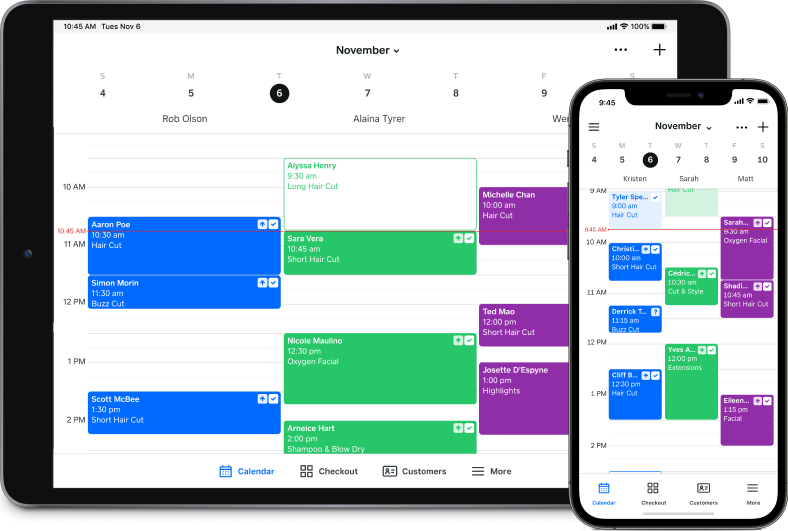
\includegraphics[width=1.0\textwidth]{content/existing_reservation_systems/square_appointments.png}
    \caption[Square Appointments]{Square Appointments~\cite{square}}
    \label{fig:square_appointments}
\end{figure}
